\documentclass[12px]{report}

%
%   Packages
%
\usepackage[a4paper,top=2cm,bottom=2cm,left=2cm,right=2cm]{geometry}
\usepackage{graphicx}
\usepackage[sorting=none]{biblatex}
\usepackage[acronym]{glossaries}
\usepackage[english]{babel}
\usepackage{csquotes}
\usepackage{setspace}

%
%   Line spacing
%
\setstretch{1.5}


%
%   Utilities and costants
%
\def\blankpage{
    \clearpage
    \thispagestyle{empty}
    \addtocounter{page}{-1}
    \null
    \clearpage
}

%
%   Acronyms
%
\newacronym{ms}{MS}{\textit{Mobile system}}
\newacronym{dos}{DOS}{\textit{Denial Of Service}}
\newacronym{iot}{IOT}{\textit{Internet Of Things}}
\newacronym{ran}{RAN}{\textit{Radio Access Network}}
\newacronym{ue}{UE}{\textit{User Equipment}}
\newacronym{bs}{BS}{\textit{Base Station}}
\newacronym{sim}{SIM}{\textit{Subscriber Identity Module}}
\newacronym{mtso}{MTSO}{\textit{Mobile Telephone Switching Office}}
\newacronym{fdma}{FDMA}{\textit{Frequency Division Multiple access}}
\newacronym{gsm}{GSM}{\textit{Global System for Mobile Communications}}
\newacronym{sms}{SMS}{\textit{Short Message Service}}
\newacronym{bss}{BSS}{\textit{Base Station Subsystem}}
\newacronym{nss}{NSS}{\textit{Network Switching Subsystem}}
\newacronym{msc}{MSC}{\textit{Mobile  Switching  Center}}
\newacronym{ptsn}{PTSN}{\textit{Public switched telephone network}}
\newacronym{hlr}{HLR}{\textit{Home Location Register}}
\newacronym{vlr}{VLR}{\textit{Visitor Location Register}}
\newacronym{eir}{EIR}{\textit{Equipment Identity Register}}
\newacronym{auc}{AuC}{\textit{Authentication Center}}
\newacronym{gprs}{GPRS}{\textit{General Packet Radio Service}}
\newacronym{sgsn}{SGSN}{\textit{Serving GPRS Support Node}}
\newacronym{wcdma}{W-CDMA}{\textit{Wideband Code Division Multiple Access}}
\newacronym{umts}{UMTS}{\textit{Universal Mobile Telecommunications System}}
\newacronym{ggsn}{GGSN}{\textit{Gateway GPRS Support Node}}
\newacronym{ip}{IP}{\textit{Internet Protocol}}
\newacronym{hss}{HSS}{\textit{Home Subscriber Server}}
\newacronym{mme}{MME}{\textit{Mobility Management Entity}}
\newacronym{sgw}{S-GW}{\textit{Serving - Gateway}}
\newacronym{lte}{LTE}{\textit{Long Term Evolution}}
\newacronym{pgw}{P-GW}{\textit{Packet data network - Gateway}}
\newacronym{pcrf}{PCRF}{\textit{Policy Control and Charging Rules Function}}
\newacronym{sba}{SBA}{\textit{Service Base Architecture}}
\newacronym{sdn}{SDN}{\textit{Software Defined Network}}
\newacronym{ddos}{DDOS}{\textit{Distributed Denial Of Service}}
\newacronym{aka}{AKA}{\textit{Authentication and Key Agreement}}
\newacronym{imsi}{IMSI}{\textit{International Mobile Subscriber Identity}}
\newacronym{imei}{IMEI}{\textit{International Mobile Equipment Identity}}
\newacronym{tmsi}{TMSI}{\textit{Temporary Mobile Subscriber Identity}}
\newacronym{sres}{SRES}{\textit{Signed Response}}
\newacronym{suci}{SUCI}{\textit{Subscription Concealed Identifier}}
\newacronym{ik}{IK}{\textit{Integrity Key}}
\newacronym{snn}{SNN}{\textit{Serving Network Name}}
\newacronym{tps}{TPS}{\textit{Transation Per Second}}
\newacronym{nfv}{NFV}{\textit{Network Functions Virtualization}}
\newacronym{mitm}{MITM}{\textit{Man In The Middle}}
\newacronym{ecies}{ECIES}{\textit{Elliptic Curve Integrated Encryption Scheme}}
\newacronym{supi}{SUPI}{\textit{Subscription Permanent Identifier}}
\newacronym{smf}{SMF}{\textit{Session Management Function}}
\newacronym{pcf}{PCF}{\textit{Policy Control Function}}
\newacronym{udm}{UDM}{\textit{Unified Data Management}}
\newacronym{ausf}{AUSF}{\textit{Authentication Server Function}}
\newacronym{sdsf}{SDSF}{\textit{Structured Data Storage Network Function}}
\newacronym{udsf}{UDSF}{\textit{Unstructured Data Storage Network Function}}
\newacronym{aria}{ARIA}{\textit{Air Pollutants Monitoring Using UAVs}}
\newacronym{cots}{COTS}{\textit{Commercial off-the-shelf}}
\newacronym{uavs}{UAVs}{\textit{Unmanned Aerial Vehicles}}
\newacronym{wsn}{WSN}{\textit{Wireless Sensor Network}}
\newacronym{epa}{EPA}{Environmnetal Protection Agengy}
\newacronym{nef}{NEF}{\textit{Network Exposure Function}}
\newacronym{nrf}{NRF}{\textit{Network Repository Function}}
\newacronym{nssf}{NSSF}{\textit{Network Slicing Selector Function}}
\newacronym{upf}{UPF}{\textit{User Plane Function}}
\newacronym{amf}{AMF}{\textit{Access and Mobility Management Function}}
\newacronym{seaf}{SEAF}{\textit{Security Anchor Function}}
\newacronym{guti}{GUTI}{\textit{Globally Unique Temporary Identifier}}
\newacronym{fach}{FACH}{\textit{Forward Access Channel}}
\newacronym{autn}{AUTN}{\textit{Authentication Token}}
\makenoidxglossaries

%
%   References
%
\addbibresource{formats/references.bib}

%
%   Document
%
\begin{document}
    \begin{titlepage}
  \begin{center}
    
\includegraphics[width=0.3\textwidth]{images/unipd.png}
    \hfill
    
\includegraphics[width=0.3\textwidth]{images/dei.png}
  \end{center}
  \begin{center}
    \vspace{3cm}
    \large
    \MakeUppercase{
      \textbf{
        Dipartimento di ingegneria dell'informazione\\
        \vspace{0.5cm}
        Corso di laurea in Ingegneria Informatica\\
      }
    }
    \vspace{4cm}
    \MakeUppercase{
      \textbf{
        Sviluppo del software di acquisizione ed elaborazione delle misure dell'inquinamento dell'aria di droni progetto A.R.I.A.\\
      }
    }
    \vspace{4cm}
    \begin{flushleft}
      \textbf{
        Relatore: Prof. Carlo Bettanini Fecia di Cossato\\
      }
    \end{flushleft}
    \vspace{1cm}
    \begin{flushright}
      \textbf{
        Laureando: Giacomo Favaron\\
      }
    \end{flushright}
    \vspace{2.5cm}
    \MakeUppercase{
      \textbf{
        Anno accademico: 2020-2021\\
      }
    }
    \vspace{0.5cm}
    \textbf{
      Data di laurea: 15/11/2021
    }
  \end{center}
\end{titlepage}
    %\blankpage
    \begin{abstract}
In the recent years, awareness of the issue of Environmental Pollution has increased, and research shows that not enough has been done, until now, to reduce pollution. In this domain, the monitoring of air quality is fundamental to provide data which can be used to most effectively guide our efforts to reduce air pollution. At this time the monitoring of air quality is usually performed via stationary ground-mounted air pollution stations. However, research(??) has shown that air pollution can vary greatly at different heights, for this reason the \gls{aria} project is aiming to develop a system to measure vertical gradients of air pollutants using vertical swarms of drones. The \gls{aria} project solution is a low-cost monitoring system based on \gls{cots} sensors and on multiple cheap drone platforms. The system is equipped with $PM_2.5$ and $PM_10$ sensors to monitor the particulate concentration and several other gas sensors (such as $NO$, $NO_2$, $CO$, etc.) and the use of \gls{uavs} allows to build a 3D map of pollutants in a specific area. This could prove very useful around buildings in urban areas and possibile polluting plants in industrial areas. In this thesis are presented the system platform, the software implementation and a test flight.
\end{abstract}
    \clearpage
    \tableofcontents{}
    \clearpage
    \listoffigures
    \clearpage
    \printnoidxglossary[type=acronym, title={List of abbreviations}, style=index, nonumberlist]
    \printacronyms
    \clearpage
    \chapter{Introduction}
% TODO:
% - Trovare ref punti di domanda
Air pollution is caused by different typologies of gas pollutants that are present in the first meters (<150 m) of the atmosphere and cause therefore damages to humans and environment. As air pollution is becoming the largest environmental health risk, the monitoring of air quality has drawn much attention in both laboratory studies and specific field tests and data collection campaigns. Government agencies and local administrations have, generally, provided and used monitoring stations on dedicated sites in cities and urban areas. Usually the studies have been conducted using fixed stations that are very reliable but produce only coarse-grained 2D monitoring, with several kilometers between two monitoring stations; or the stations monitor the same local area for long periods.
Other approaches show that applications using simple system of sensors have been developed to monitor the fine-grained air quality using densely deployed sensors [? ], [? ]. In any case, the fixed sensor station may achieve high precision, but have high cost and require maintenance and suffer especially for lack of mobility.
Furthermore, these approaches don't account for the vertical gradients of air pollution levels. As shown in research (?, ?) the concentrations of air pollutants can vary greatly at different heights and this is a sensitive factor in circumstances such as buildings in urban areas and possible polluting plants in industrial areas.
The usage of Unmanned Aerial Vehicles (UAVs) has been particularly rich in the latest years due to their flexibility, mobility and affordable cost. Current monitoring systems are not able to satisfy every need of modern cities and industrial areas and UAVs are valuable supporting elements in this scenario.
In terms of urban conditions, which is the main subject of the present study, UAVs can be used to measure environmental parameters such as illumination, wind speed, temperature, humidity, air quality [? ] and much more. In any case, for a complete analysis, both ground sensing and aerial sensing are necessary to provide 3D mapping and gas profiling. In our ARIA project, we equipped with the same set of sensors the devices that execute sensing on the ground, and the systems that execute aerial sensing on board the \gls{uavs}.
%, which we are exploring to deploy in vertical swarms, to measure pollution levels at different heights.
The fixed ground sensing suite is able to collect data in a continuous way, but the air quality of the higher levels of air off the ground cannot be detected, so the contemporary use of drones is mandatory. Aerial sensing, on the contrary, is able to sense the air quality off the ground, but it cannot be executed for very long periods due to the high consumption of battery power and human time. By merging the potentialities of these two systems of sensing suites, a better set of data can be collected [? ]. A trade off on the possible sensors and UAVs has been performed and quadcopters are the preferred platform for monitoring because of their simplicity, low cost and hovering capabilities. On the contrary a possible bias of data is due to the the influence of air jets created by the rotor rotation or by the electromagnetic field generated by the antennas present on board. The problem of choosing the best location of the sensors is examined in [? ] based on the physical structure of the drones. Our approach is to use an extension on which we fix the sensors in order to suck the air away of the main air jets.

ARIA project was created by a group of students from the Department of Industrial Engineering, University of Padova, under the suggestion and guidance of personnel staff of the Center for Space Studies and Activities (CISAS) of the same University. The core motivation that brought together these students was the desire of researching new fields of application for drone technology. ARIA project has been carried on figuring this scenario: air quality monitoring.
\section{Related works and state of the art}
\subsection{Air Pollution}
Air pollution is extremely complex to evaluate and there are many polluting substances in the atmosphere. The \gls{epa} (of United States) takes these 6 in consideration in its studies:
\begin{center}
\begin{tabular}{ |c|c|c| }
    \hline
    Chemical symbol & Substance & Characteristics \\ [0.5ex]
    \hline
    CO & Carobon Monoxide & Colorless, odorless gas \\
    $NO_2$ & Nitrogen Dioxide & Highly reactive gas \\
    $O_3$ & Ozone & Pale blue gas \\
    $SO_2$ & Sulfur Dioxide & Colorless, irritating smell gas \\
    $PM_2.5$ and $PM_10$ & Particulate Matter & Inhalable particles \\
    Pb & Lead & Metal particles \\
\end{tabular}
\end{center}
\subsection{Low-cost sensors}
The \gls{epa} also provides the Air Sensor Guidebook\cite{williams2014-air} which gives extensive information on air quality and low-cost sensors.

\cite{evangelatos2015airborne}, \cite{8675167}, \cite{8662050} propose different implementation of a \gls{wsn} using \gls{uavs}. The differentiating factor of the \gls{aria} project solution is the use of vertical swarms to monitor pollution at different heights, which is not a popular topic.
\section{Dissertation structure}
This dissertation describes the \gls{aria} project solution for the monitoring of air pollution. It is divided into 6 chapters:
\begin{itemize}
    \item Chapter 1 describes the introduction, an overview on the topic of air pollution, the motivation to approach the problem, the motivation of the proposed solution, related works, the state of the art and the dissertation objective.
    \item Chapter 2 describes the system architecture, that is the \gls{uavs} that are being used, their design, specifications and functionality.
    \item Chapter 3 describes the sensor payload, the motivation of the adopted sensors and their use.
    \item Chapter 4 describes the software implementation for the data collection of the sensors and the communication of the \gls{uavs}.
    \item Chapter 5 shows the results of a test flight using the proposed solution.
    \item Chapter 6 presents what conclusions can be taken after all the developed work, and what improvements can be done in the future.
\end{itemize}
\section{Dissertation objective}
The objective of this dissertation is to describe the solution proposed by the \gls{aria} project for air pollution monitoring, in particular the software impelementation, to show preliminary results and discuss their revelance in future applications.
    \clearpage
    \chapter{ARIA: System architecture}

    \clearpage
    \chapter{Generazioni cellulari}
Nel corso degli anni, si sono susseguite diverse generazioni di tecnologie cellulari che hanno apportato
notevoli cambiamenti alla loro architettura e infrastruttura per consentire il raggiungimento di prestazioni migliori\cite{architecture-evolution}.\\
Di seguito verranno presentate le principali caratteristiche
delle diverse generazioni cellulari, in modo tale da rendere di facile comprensione l'analisi dei meccanismi
di autenticazione che verranno approfonditi nelle prossime sezioni.\\
Oltre ad elencare le principali caratteristiche di ogni generazione verranno analizzate nel dettaglio le specifiche  
delle architetture.
\begin{figure}[ht]
    \centering
    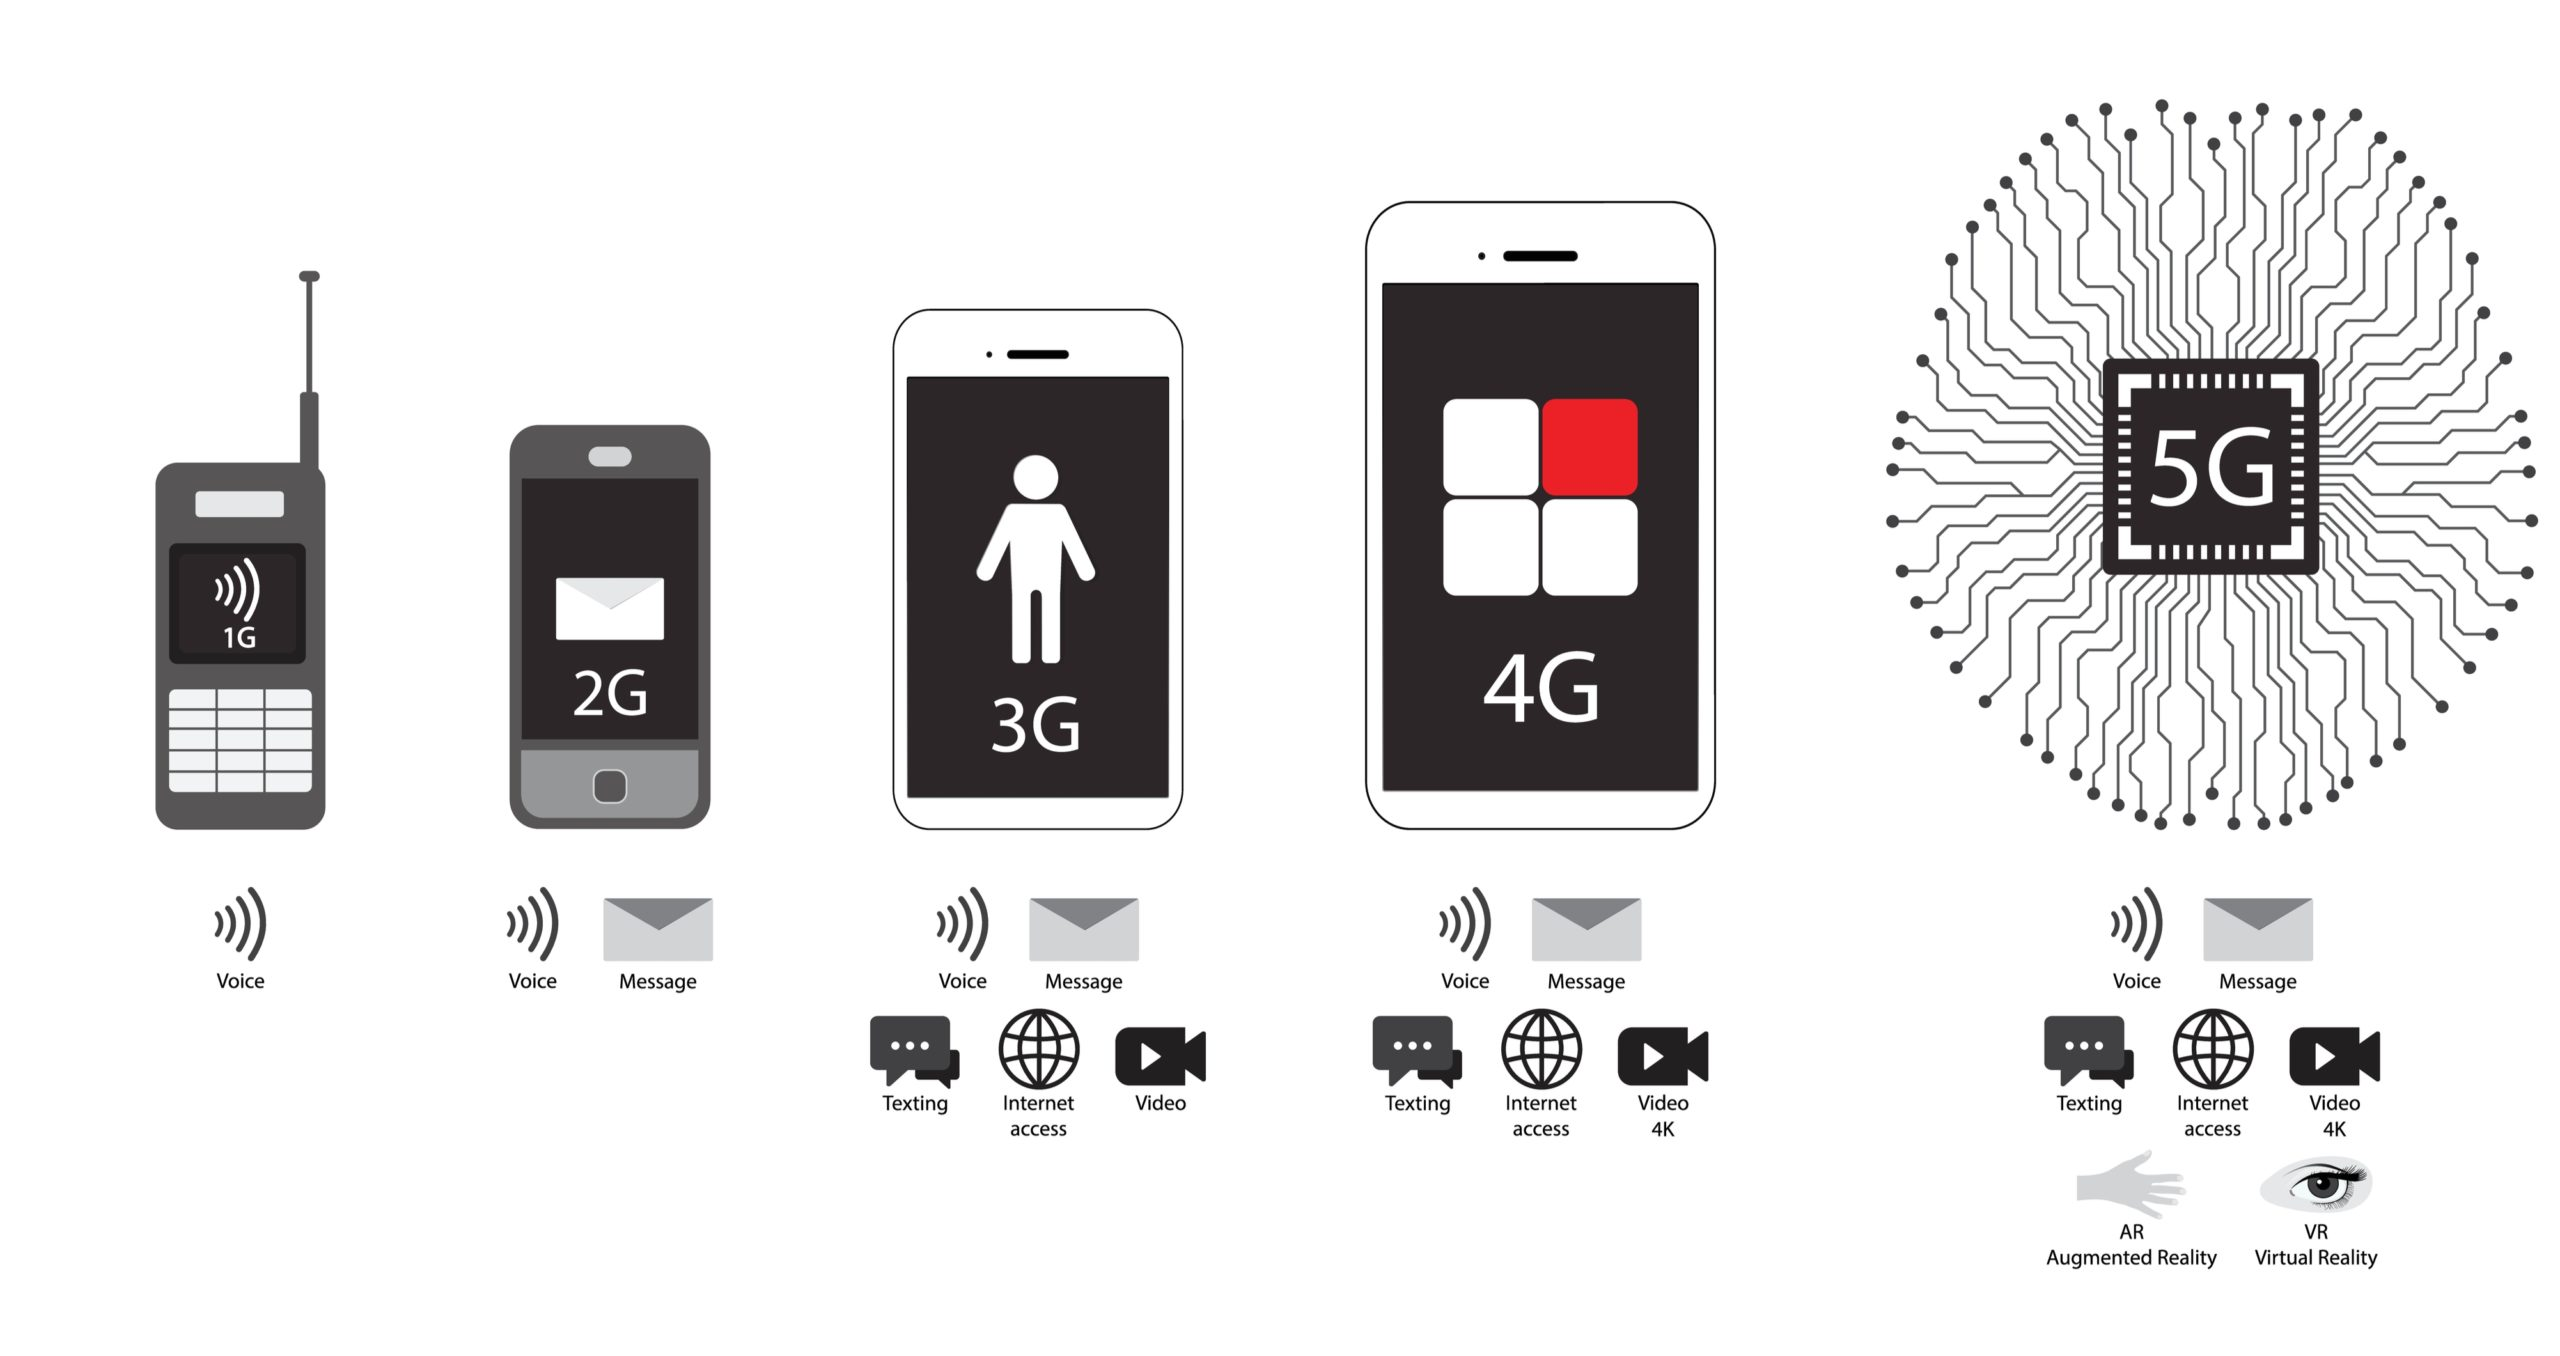
\includegraphics[width=0.7\textwidth]{images/generations-scheme.jpg}
    \caption{Schema delle generazioni cellulari}
\end{figure}

\clearpage

\section{1G}
La generazione 1G è uno dei primi standard di comunicazione cellulare. Il suo funzionamento era completamente analogico 
e ormai è stata rimpiazzata totalmente dalle generazioni digitali successive.\\
L'architettura di questa generazione è molto semplice, è composta da tre componenti principali:
\begin{itemize}
    \item Antenne per la trasmissione
    \item \gls{mtso}
    \item Unità mobile (cellulare)
\end{itemize}
\begin{figure}[ht]
    \centering
    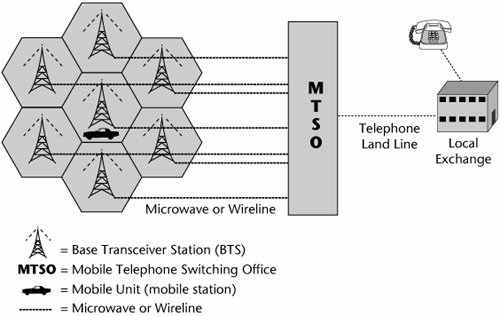
\includegraphics[width=0.7\textwidth]{images/1g.jpg}
    \caption{Architettura 1G}
\end{figure}
Si basava sulla \gls{fdma} in cui ogni dispositivo che si connetteva alla stazione radio
aveva assegnata una specifica sotto banda\cite{generations}.

\clearpage

\section{2G}
A differenza della prima generazione, la seconda introuduce per la prima volta una rete completamente digitale.
Questa tecnologia cellulare è composta da diverse versioni che si sono susseguite nel corso degli anni aggiungendo nuove 
funzionalità.
Anche la sua architettura subisce delle modifiche, per questo verranno trattate separatamente in seguito.
\subsubsection{GSM}
Il \gls{gsm}\cite{gsm} è uno standard di seconda generazione che introuduce importanti novità.\\
Le principali caratteristiche introdotte sono:
\begin{itemize}
    \item Maggiori velocità di trasmissione
    \item Cifratura della comunicazione
    \item Introduzione di nuovi servizi come gli \gls{sms}
\end{itemize}
\begin{figure}[ht]
    \centering
    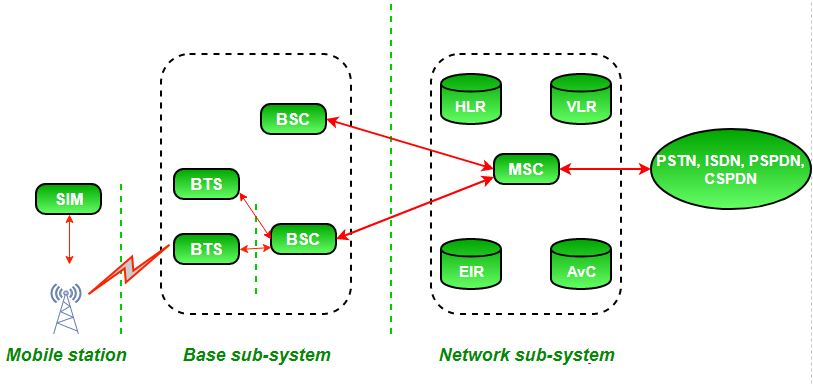
\includegraphics[width=0.7\textwidth]{images/2g-gsm.jpg}
    \caption{Architettura GSM}
\end{figure}
La sua architettura è composta da due macro aree: La \gls{bss} e la \gls{nss}.
Il \gls{bss} è l'insieme delle antenne ricevitori che rappresentano il primo collegamento con il \gls{ms}, mentre il \gls{nss} rappresenta il \textit{core network} del \gls{gsm}.\\
Il \gls{nss} è formato dai seguenti componenti:
\begin{itemize}
    \item \gls{msc} è l'elemento centrale dell'atchitettura \gls{gsm}, si occupa di interfacciare le \gls{bs} con la rete telefonica \gls{ptsn}.
    \item \gls{hlr} \textit{database} centrale che contiene informazioni inerenti a tutti i \textit{subscribers}, molte delle informazioni
    che contiene sono dei puntatori agli archivi seguenti.
    \item \gls{vlr} \textit{database} che memorizza la posizione degli utenti.
    \item \gls{eir} \textit{database} degli \gls{imei} dei dispositivi. Grazie a questo archivio è possibile creare delle \textit{blacklist}
    per evitare l'accesso a determinati terminali.
    \item \gls{auc} \textit{database} delle informazioni di sicurezza associate agli utenti registrati.
\end{itemize}

\clearpage

\subsection{GPRS}
La rete \gls{gprs}\cite{gprs-edge} introduce per la prima volta un trasferimento dati a commutazione di pacchetto per rendere 
possibile l'utilizzo dei servizi \textit{internet} con il proprio dispositivo cellulare\cite{gsm-architecture}.
La sua architettura è la stessa di quella del \gls{gsm} ma con dei componenti aggiuntivi che consentono la trasmissione dei pacchetti. 
Per esempio, il \gls{sgsn} è un componente per la gestione dei dispositivi connessi alla rete.
\begin{figure}[ht]
    \centering
    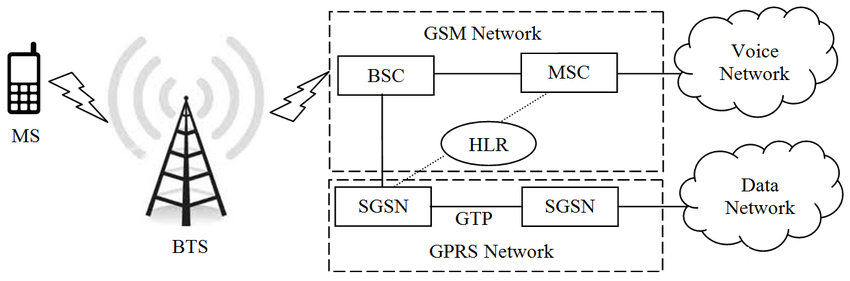
\includegraphics[width=0.7\textwidth]{images/2g-gprs.png}
    \caption{Architettura GPRS}
\end{figure}
\subsection{EDGE}
Evoluzione del \gls{gprs} che consente maggiori velocità, l'architettura resta invariata\cite{gprs-edge}.

\clearpage

\section{3G}
L'architettura della terza generazione riprende quella già vista nella seconda. Infatti, questa generazione ha avuto come principale obbiettivo 
quello di consolidare l'integrazione della rete internet nei sistemi cellulari ed aumentare la velocità di trasmissione per consentire l'utilizzo 
di nuovi servizi.\\
L'accesso al canale radio avviene con la tecnologia \gls{wcdma} con canale di banda 5 MHz.

\subsection{UMTS}
Lo \gls{umts} è il primo standard di terza generazione.
La sua architettura è composta dai seguenti elementi principali:
\begin{itemize}
    \item \gls{msc}, componente che ha la stessa funzione di quello in 2G. Questa volta il \gls{vlr} è integrato al suo interno.
    \item \gls{hlr}/\gls{auc} e \gls{eir}
    \item \gls{sgsn} e \gls{ggsn} ovvero dei componenti ripresi dalla rete \gls{gprs} per la commutazione a pacchetto.
\end{itemize}
\begin{figure}[ht]
    \centering
    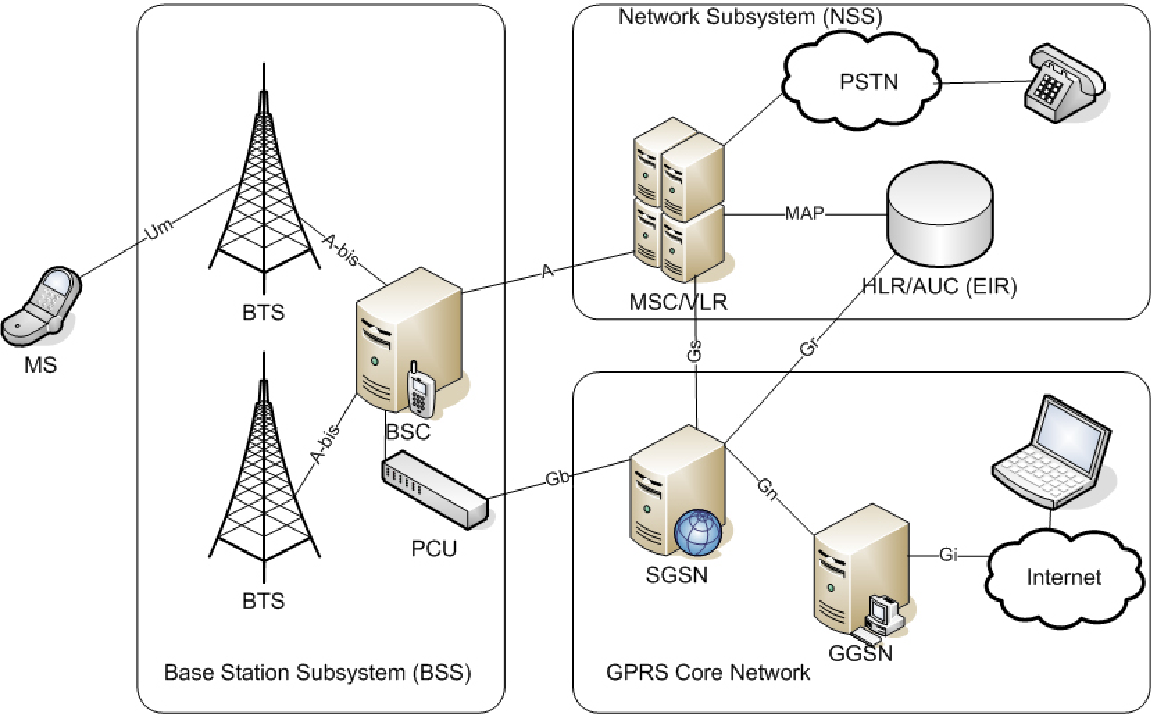
\includegraphics[width=0.7\textwidth]{images/3g-umts.png}
    \caption{Architettura UMTS}
\end{figure}


\subsection{HSPA/HSPA+}
Evoluzione del \gls{umts} per consentire velocità maggiori apportando modifiche nella trasmissione del segnale.
Con questo nuovo standard si riescono a raggiungere velocità di 42 Mb/s\cite{hspa}.

\clearpage

\section{4G}
La quarta generazione è al momento quella più utilizzata, permette di avere dei servizi basati su velocità molto alte. 
A differenza delle precedenti generazioni che dovevano gestire due \textit{core network}: uno per la rete telefonica e un altro
per \textit{internet}, per la prima volta il 4G introduce un unico \textit{core network} basato su \gls{ip}.\\
Per consentire un aumento consistente della velocità, le maggiori modifiche di questa generazione sono state apportate nella \textit{radio interface}, mentre
l'architettura rimane con una struttura simile a quella precedente.
\subsection{LTE}
la \gls{lte} è uno standard di quarta generazione che ha i seguenti componenti architetturali\cite{lte}:
\begin{itemize}
    \item \gls{hss} è il \textit{database} centrale dei \textit{subscriber} come l'\gls{hlr} del \gls{gsm}/\gls{umts}.
    \item \gls{mme} è il corrispettivo del \gls{vlr} in \gls{gsm}/\gls{umts}.
    \item \gls{sgw} è un componente che svolge il ruolo di \textit{router} indirizzando i dati dalla \textit{base station}
    al P-GW.
    \item \gls{pgw} è il componente per interfacciare il \textit{core network} con \textit{internet}.
    \item \gls{pcrf} è un componente responsabile delle regole di gestione per il flusso di informazioni.
\end{itemize}
\begin{figure}[ht]
    \centering
    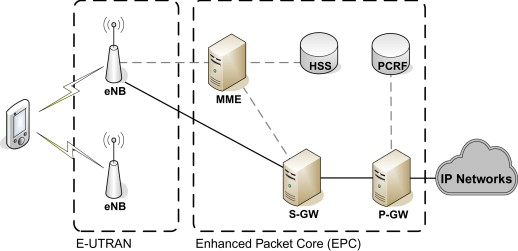
\includegraphics[width=0.8\textwidth]{images/4g-lte.jpg}
    \caption{Architettura LTE}
\end{figure}

\clearpage

\section{5G}
Il 5G, ovvero lo standard di quinta generazione rappresenta l'ultima frontiera della tecnologia cellulare.
Il suo principale scopo è consentire lo \gls{iot} massivo, ossia un \textit{network} che sia 
in grado di gestire la connessione di molti dispositivi con latenze molto piccole.
Per consentire velocità fino a 10 Gb/s si sono
dovute apportare importanti modifiche strutturali che rendono la sua architettura molto diversa da quelle viste fin'ora.\\
L'architettura implementata prende il nome di \gls{sba}.
La \gls{sba} consiste nel dividere tutti i componenti architetturali in una serie di \textit{microservices}\cite{5g-approach}. 
Questa nuova struttura è stata introdotta per garantire la scalabilità del sistema, migliorare le prestazioni (velocità) e per 
permettere la gestione simultanea di molti dispositivi.\\
I principali elementi che la compongono sono:
\begin{itemize}
    \item \gls{amf} responsabile dell'autenticazione e localizzazione del dispositivo.
    \item \gls{smf} per la gestione della sessione di ogni \gls{ms}.
    \item \gls{pcf} per la gestione delle \textit{policy}.
    \item \gls{udm} per la gestione dell'identità dell'utente, questo compito era precedentemente svolto da \gls{hss} o \gls{hlr}.
    \item \gls{ausf} per effettuare l'autenticazione dell'utente.
    \item \gls{sdsf} è un helper per la memorizzazione di dati strutturati.
    \item \gls{udsf} è un helper per la memorizzazione di dati non strutturati.
    \item \gls{nef} per esporre determinate funzionalità a servizi di terze parti.
    \item \gls{nrf} per scoprire tutti i servizi disponibili.
    \item \gls{nssf} per selezionare una determinata partizione di \textit{network}.
    \item \gls{upf} trasporta il traffico dal \gls{ran} all'internet.
\end{itemize}
\begin{figure}[ht]
    \centering
    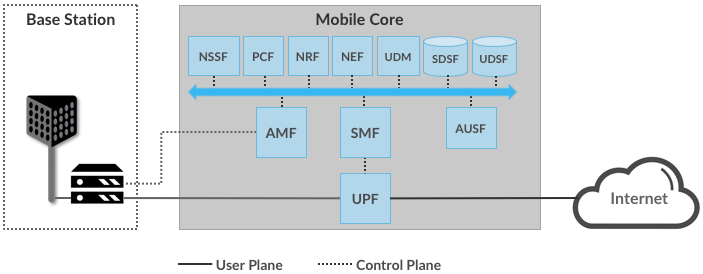
\includegraphics[width=0.8\textwidth]{images/5g-planes.png}
    \caption{Architettura 5G\cite{5g-approach}}
\end{figure}

\clearpage

\subsection{Network Slicing}
Il \textit{Network Slicing} rappresenta una delle caratteristiche più importanti del 5G. Con questo termine si intende il partizionamento della
rete in diversi "piani" ciascuno con caratteristiche e requisiti particolari, indipendente e autonomo. Questo risulta fondamentale nella realizzazione 
dell' \gls{iot} massivo, infatti in questo modo la gestione del traffico terrà conto dell'applicazione che viene utilizzata nel dispositivo per decidere di quali prestazioni di rete ha bisogno. 
\begin{figure}[ht]
    \centering
    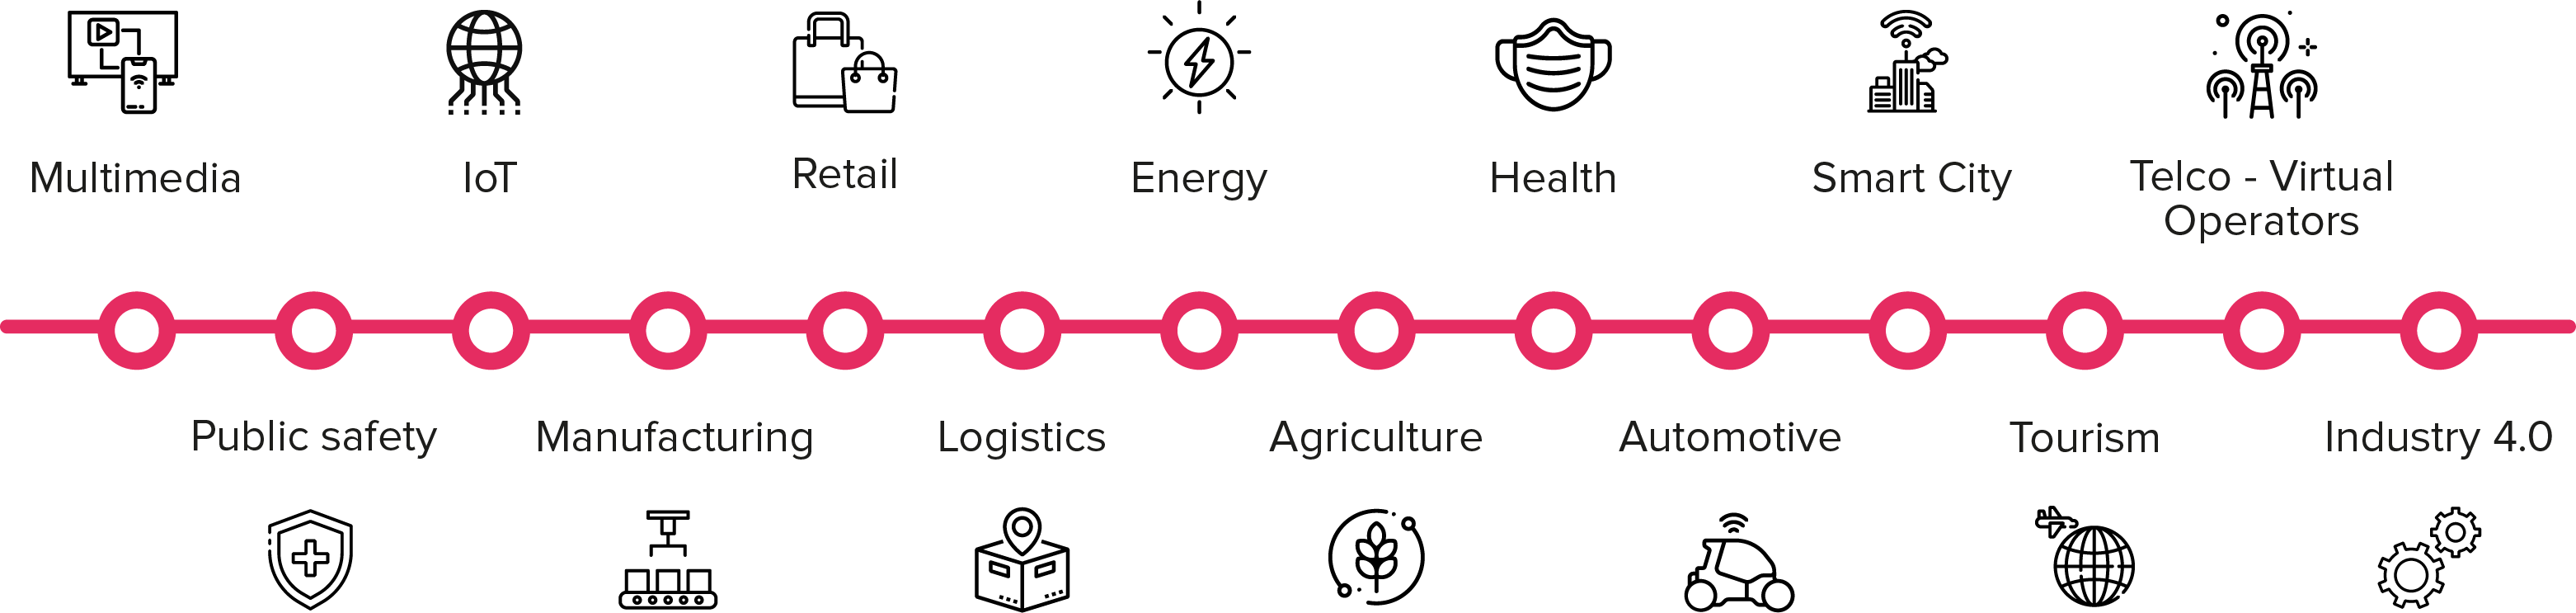
\includegraphics[width=0.8\textwidth]{images/5g-eg-of-use.png}
    \caption{Esempi di applicazioni per il 5G}
\end{figure}\\
Ogni segmento virtuale del \textit{network} ha uno specifico identificativo che deve essere indicato nella fase di autenticazione come verrà illustrato nella sezione 5.3. Per ogni \textit{slice} sono 
richieste delle prestazioni differenti, per esempio il settore delle \textit{critical communication} deve avere delle latenze molto basse.
\begin{figure}[ht]
    \centering
    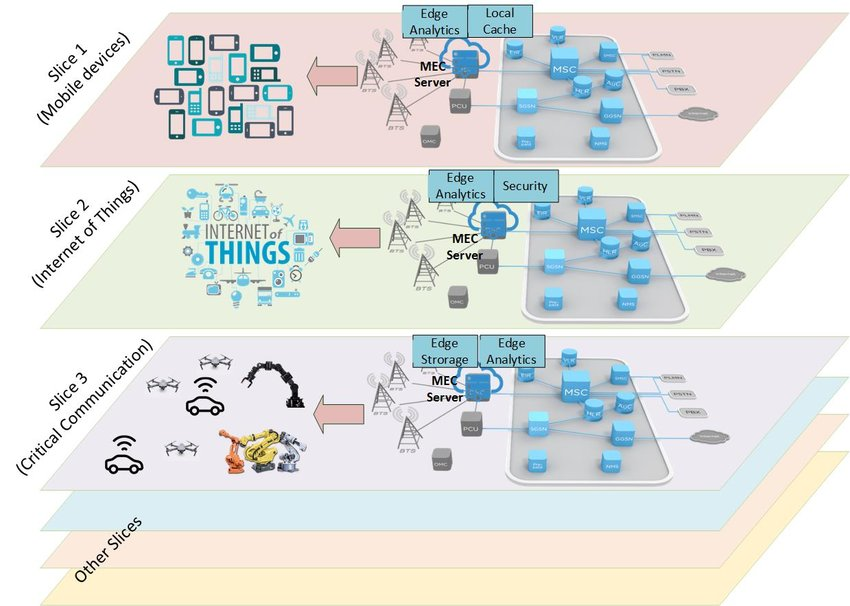
\includegraphics[width=0.8\textwidth]{images/5g-slicing.jpg}
    \caption{\textit{Network slicing} nel 5G}
\end{figure}\\
La realizzazione del \textit{Network Slicing} avviene tramite il paradigma del \textit{Software Defined Network} che nella prossima sezione verrà approfondito.

\clearpage

\subsection{\textit{Software Defined Network} e  \textit{Network Functions Virtualization}}
Il \gls{sdn} è un paradigma per gestire il \textit{network} in modo efficace. 
In questo caso il \textit{network} è definito da \gls{nfv}, dove intere classi di funzioni sono virtualizzate.
Questi sono necessari per interfacciarsi a livello applicativo con i dispositivi cellulari 
in modo da gestire il traffico della rete in modo efficace\cite{5g-sdn}.
    \clearpage
    \chapter{Attacco Denial of Service}
L'attacco di tipo \gls{dos} consiste nel rendere non disponibili servizi offerti da computer o altri
dispositivi \cite{dos-definition}. Questo avviene esasperando di richieste la macchina o l'infrastruttura che viene scelta come
vittima.

\section{Vulnerabilità nelle reti cellulari}
Le reti cellulari non sono esenti da questo tipo di attacchi, anzi, sono uno degli obiettivi più ambiti poichè essenziali per la vita quotidiana.
Sono diversi i componenti che possono essere vulnerabili a un attacco DOS in una rete cellulare. Gli obiettivi identificati come ottimi sono quelli
che comportano un maggior utilizzo delle risorse computazionali della rete.\\
Nelle prossime sezioni verranno illustrate le principali metodologie per fare un attacco di tipo \gls{dos} alle reti cellulari\cite{4g-dos-recap}.

\clearpage

\subsection{Radio Jamming}
Il \textit{Radio Jamming} è una tipologia di attacco \gls{dos} che consiste nel disturbare il segnale cellulare emettendo delle onde radio.
La realizzazione di questo tipo di attacco è molto semplice, basta procurarsi un trasmettitore che invia segnali ad alta energia nella banda cellulare di riferimento.\\
Un miglioramento del classico \textit{radio jamming} è lo \textit{smart jamming} che consiste nel saturare uno o più canali di comunicazione della rete. Questo fa sembrare 
il \textit{network} non disponibile a tutti gli utenti collegati a quella determinata cella.
\begin{figure}[h]
    \centering
    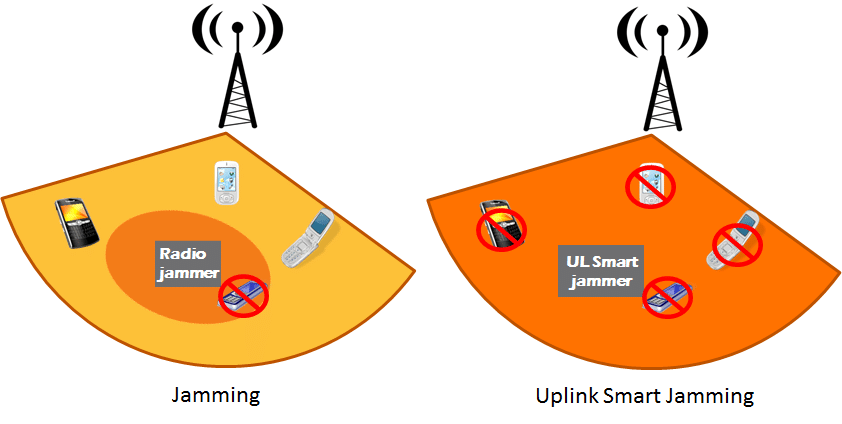
\includegraphics[width=0.6\textwidth]{images/dos-jamming.png}
    \caption{\textit{Radio} e \textit{smart jamming}\cite{4g-dos-recap}}
\end{figure}\\

\subsection{Vulnerabilità di sistema}
Un altro classico modo per creare un interruzione di sistema in una rete cellulare è sfruttando le classiche vulnerabilità che si presentano spesso in qualsiasi tipo di computer.
Questo ovviamente perchè tutta l'architettura di una rete cellulare non è altro che \textit{server} con specifiche particolari.

\subsection{Botnet}
La \textit{botnet} è sicuramente una delle tipologie più diffuse, ed è il modo con cui si realizzano i \gls{ddos}. L'attaccante, in questo caso, dispone del controllo di 
un grande numero di dispositivi infettati da \textit{malware} che li rendono essere controllabili da remoto per esasperare di richieste un determinato servizio.
\begin{figure}[h]
    \centering
    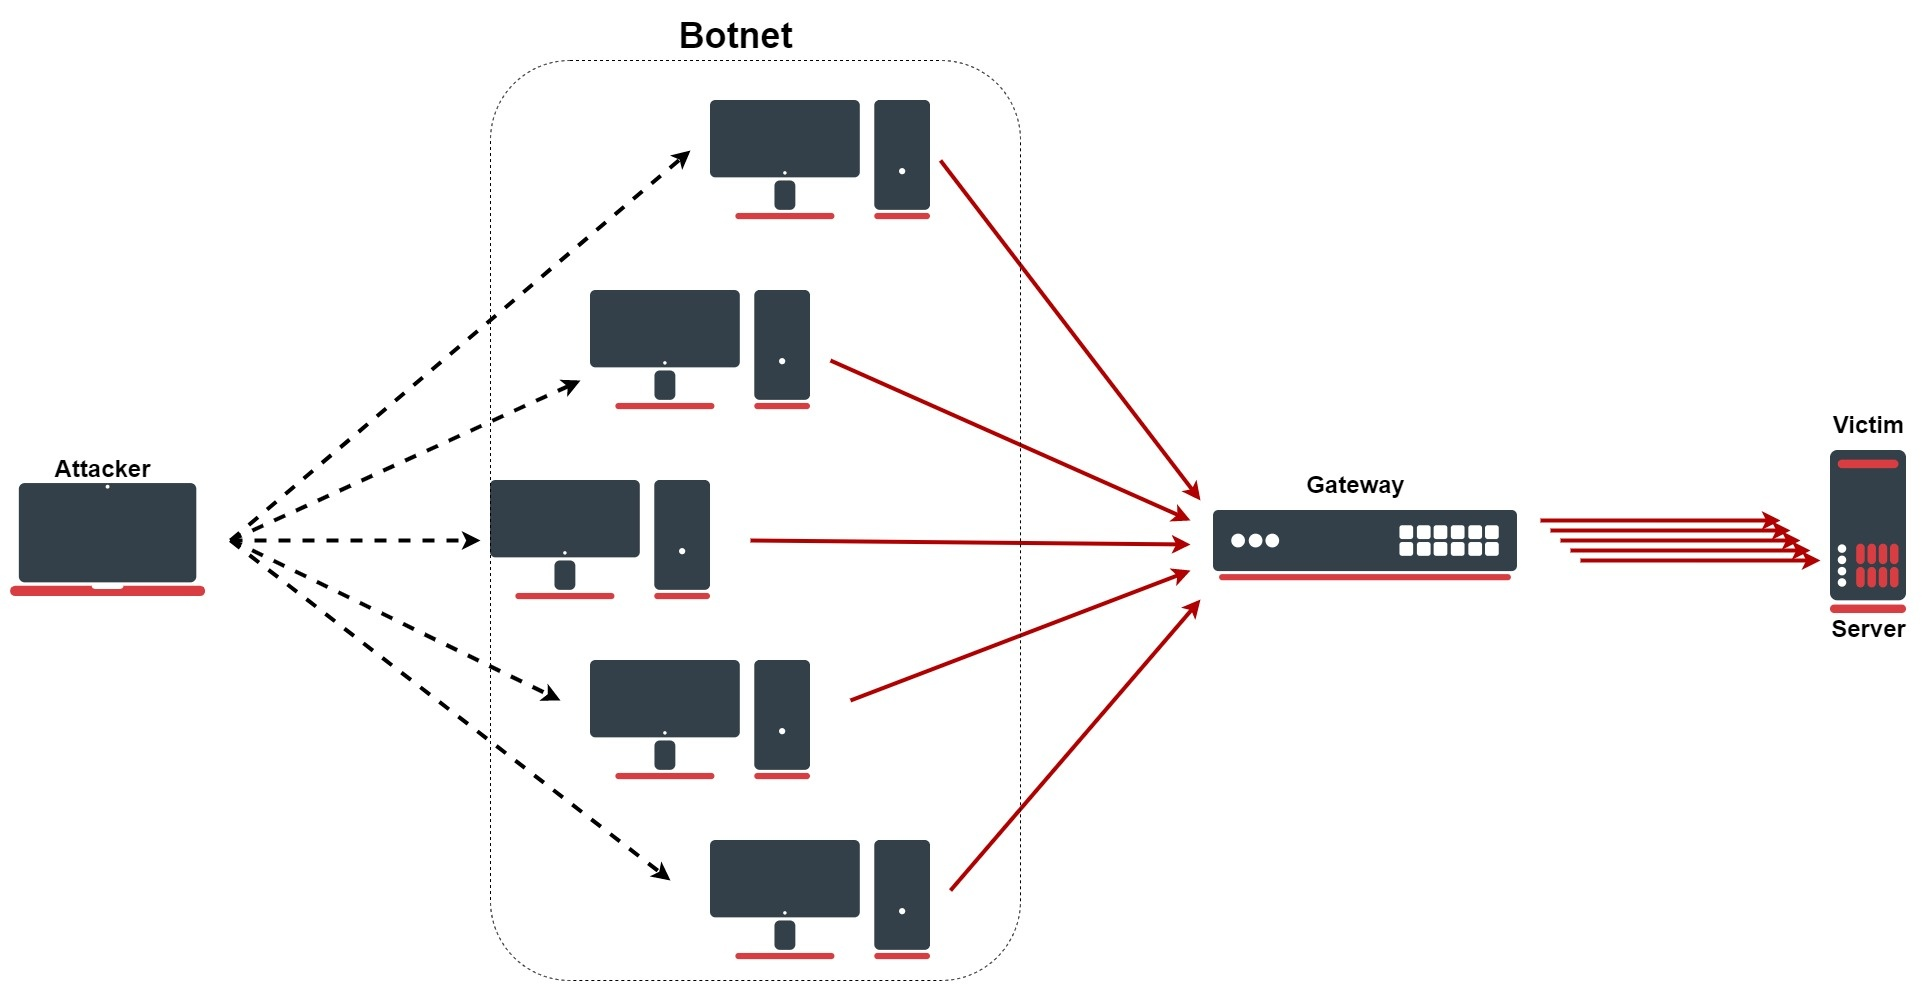
\includegraphics[width=0.5\textwidth]{images/ddos.jpg}
    \caption{\textit{Distributed denial of service}}
\end{figure}\\

\subsection{Autenticazione}
Questo è uno degli attacchi più pericolosi poichè le vulnerabilità che sfrutta sono molto difficili da risolvere dato che sono intrinseche nell'architettura del sistema.
È la tipologia di vulnerabilità che è stata scelta per confrontare la sicurezza dell'architettura 5G con quelle precedenti.
Il suo funzionamento si basa sull'esasperare di richieste di autenticazione i sistemi identificativi delle reti cellulari, che solitamente 
sono gli elementi con più traffico della rete come la HLR nelle reti 2G/3G.\\
Questa vulnerabilità si trova nel meccanismo di autenticazione dei dispositivi denominato \gls{aka} dove un dispositivo
non autenticato forza delle computazioni all'interno del \textit{core network} che consumano più risorse della richiesta stessa\cite{umts-dos}.
Ad aumentare la pericolosità di questa vulnerabilità vi è la possibilità di creare computazioni nel \textit{core network} 
senza disporre di una \gls{sim} valida. Questa tipologia di attacchi, definiti come SIM-less, verranno presi come riferimento per effettuare un attacco \gls{dos} alle 
reti \gls{gsm}\cite{gsm-dos-simless} e \gls{umts}\cite{umts-dos}.



\section{Misurazione}
Per capire quale componente della rete sia il più vulnerabile a un attacco \gls{dos} si devono fare delle misurazioni sui vari componenti del \textit{network}.
In questo modo è possibile capire in quale punto si possono creare dei rallentamenti o \textit{bottleneck} dovuti a un sovraffollamento di richieste.\\
In \cite{measuring-dos} vi è una dettagliata spiegazione di come procedere con queste misurazioni e soprattutto come quantificare il numero di dispositivi che 
servono all'attaccante per completare l'attacco con successo.\\
Solitamente le statistiche riguardo alle prestazioni dei componenti del \textit{network} non sono direttamente fornite dagli operatori telefonici quindi bisogna 
basarsi sui tempi di risposta delle misurazioni. Per esempio, l'immagine seguente mostra i tempi di risposta della \gls{hlr} in una rete \gls{umts} al comando \textit{location updates}.
\begin{figure}[h]
    \centering
    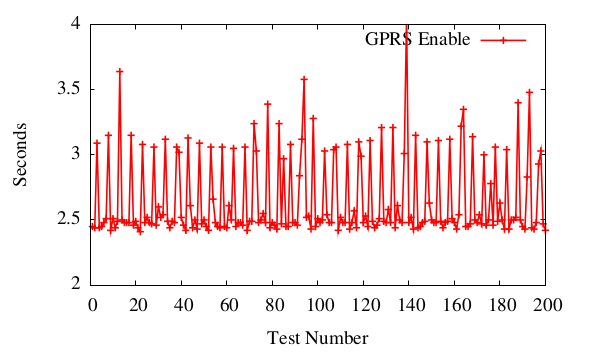
\includegraphics[width=0.7\textwidth]{images/hlr-measuring.png}
    \caption{Misurazione tempi di risposta HLR con \textit{location updates}\cite{measuring-dos}}
\end{figure}
    \clearpage
    \chapter{Sistema di autenticazione}
Il meccanismo di autenticazione è la procedura per verificare che un determinato dispositivo
sia abilitato a connettersi alla rete.
Questo procedimento avviene tramite l'\gls{aka}, procedimento in cui
il \textit{core network} abilita un dispositivo a connettersi.\\
In questo capitolo verranno trattate le procedure di autenticazione\cite{identifications} per le generazioni dal 2G al 5G, il 1G è stato escluso 
poiché ha un funzionamento completamente analogico.

\clearpage

\section{2G}
Il sistema di autenticazione di seconda generazione utilizza principalmente due codici univoci della \gls{sim} e del \gls{ms}:
\begin{itemize}
    \item \gls{imsi} ovvero un codice identificatvo della \gls{sim}.
    \item \gls{imei} ovvero un codice identificativo del \gls{ms}.
\end{itemize}
Questi due codici saranno necessari anche per le prossime generazioni fino al 4G.\\
La procedura di autenticazione di un \gls{ms} segue questi passaggi:
\begin{enumerate}
    \item Il \gls{ms} invia l'\gls{imsi} alla \gls{bs} di riferimento che lo inoltra al \textit{core network}, questo
    avviene ogni volta che il \gls{ms} vuole connettersi al \textit{network} e non risulta già registrato presso 
    la rete di riferimento. In caso lo fosse, verrà utilizzato il \gls{tmsi}
    per preservare il suo anonimato.
    \item L'\gls{auc} cerca la chiave Ki associata all'\gls{imsi} e insieme a un numero casuale RAND genera un codice \gls{sres} che verrà
    salvato nel \gls{vlr}.
    \item Viene inviato al \gls{ms} il RAND generato.
    \item La stessa procedura viene fatta dal \gls{ms}, che genera quindi il suo \gls{sres} e lo invia al \gls{vlr}.
    \item Il \gls{vlr} confronta se l'\gls{sres} ricevuto corrisponde a quello generato dall'\gls{auc}, se corrispondono l'autenticazione risulta
    effettuata con successo.
\end{enumerate}

\begin{figure}[h]
    \centering
    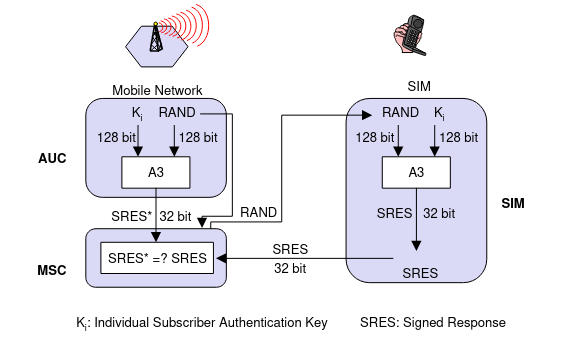
\includegraphics[width=0.7\textwidth]{images/auth-2g.png}
    \caption{Autenticazione nelle reti 2G}
\end{figure}

\clearpage

\section{3G e 4G}
Dato che l'autenticazione nelle reti 3G e 4G è molto simile, verranno trattate insieme in questa sezione.
L'autenticazione nell'architettura di terza e quarta generazione è molto simile a quella della seconda salvo i seguenti miglioramenti:
\begin{itemize}
    \item Viene introdotta l'autenticazione mutua per prevenire l'autenticazione a false \textit{base stations}.
    \item La lunghezza della chiave Ki viene incrementata da 64 a 128 bit.
    \item Viene implementato un flag per verificare se le comunicazioni vengono compromesse durante la trasmissione chiamato \gls{ik}.
\end{itemize}
Il procedimento di autenticazione è il seguente\cite{4g-auth}:
\begin{enumerate}
    \item Il \gls{ms} invia l'\gls{imsi} alla \gls{bs} di riferimento che lo inoltra al \textit{core network}.
    \item L'\gls{auc} cerca la chiave Ki associata all'\gls{imsi} e insieme a un numero casuale RAND genera un codice \gls{sres} che verrà
    salvato nel \gls{vlr}.
    \item Viene trovata la chiave Ki corrispondente all'\gls{imsi} dall'\gls{auc}, dopodichè viene generato un codice \gls{sres} con l'utilizzo di un numero randomico RAND.
    Inoltre, viene generato un codice \gls{autn} per permettere al MS di autenticare il \textit{network}.
    \item Viene inviato al \gls{ms} il RAND e \gls{autn}.
    \item Il \gls{ms} autentica il \textit{network} confrontando il valore di \gls{autn} ricevuto. Se il \textit{network} è valido, prosegue con la generazione del \gls{sres}.
    \item Il \gls{vlr} confronta se il SRES ricevuto corrisponde a quello generato dall'\gls{auc}, se corrispondono l'autenticazione risulta
    effettuata con successo e viene attribuito il \gls{tmsi} al \gls{ms}.
\end{enumerate}
\begin{figure}[h]
    \centering
    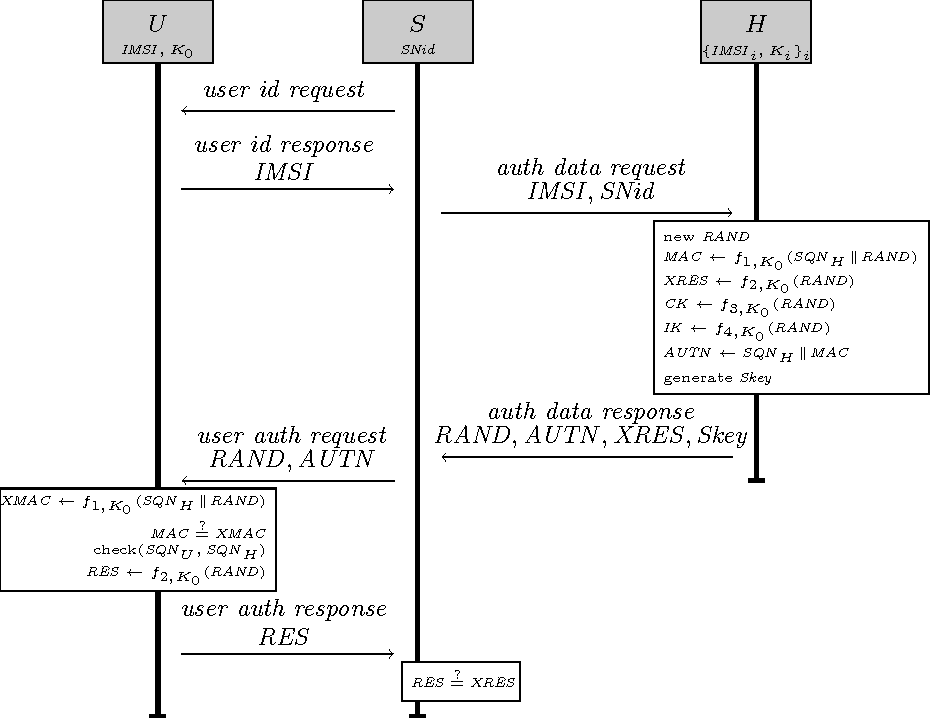
\includegraphics[width=0.7\textwidth]{images/auth-3g.png}
    \caption{Autenticazione nelle reti 3G e 4G}
\end{figure}

\clearpage

\section{5G}
L'autenticazione della generazione 5G è molto diversa dalle precedenti poichè, come illustrato nella sezione 3.5, l'architettura è completamente rivista diventando una ramificazione di microservizi.
Sono definiti tre protocolli di autenticazione:
\begin{itemize}
    \item 5G-AKA: 5G-\textit{Authentication and Key Management}.
    \item EAP-AKA: \textit{Extensible Authentication Protocol – Authentication and Key Management}.
    \item EAP-TLS: \textit{Extensible Authentication Protocol – Transport Layer Security}.
\end{itemize}
Rispetto alle generazioni precedenti ci sono stati i seguenti miglioramenti di sicurezza\cite{5g-vs-4g}:
\begin{itemize}
    \item L'\gls{imsi} non viene mai comunicato in chiaro ma sempre criptato.
    \item I componenti del \textit{network} coinvolti sono dei servizi.
\end{itemize}
L'autenticazione è divisa in due parti: La prima è l'inizializzazione dell'autenticazione e la scelta del metodo di autenticazione.
La seconda è invece l'autenticazione mutua come avviene nelle generazioni precedenti.
Lo schema di autenticazione è il seguente\cite{5g-auth}:
\begin{enumerate}
    \item Il \gls{ms} invia il \gls{suci} o 5G-GUTI alla \gls{bs} di riferimento che lo inoltra al \gls{amf} o \gls{seaf},
    il \gls{guti} è un identificativo temporaneo simile al \gls{tmsi} delle generazioni precedenti, invece il \gls{suci} è un identificatore criptato
    permanente.
    \item il \gls{seaf} manda l'identificatore del dispositivo (\gls{suci} o 5G-GUTI) e il \gls{snn} all'\gls{ausf}.
    Il \gls{snn} è una concatenazione di codici identificativi di servizi e il codice identificativo del \textit{serving network}. Serve per capire 
    a quale \textit{slice} vuole connettersi il dispositivo.
    \item L'\gls{ausf} controlla che la richiesta dal \gls{seaf} sia autorizzata a utilizzare il \gls{snn}, in caso non lo fosse risponde con un 
    apposito messaggio di errore.
    \item L'\gls{ausf} reperisce la chiave associata all'identificativo nell'archivio \gls{udm} e genera il rispettivo \gls{sres} con un numero randomico RAND.
    \item Viene inviato all'\gls{ms} il RAND e \gls{autn} (per l'autenticazione mutua).
    \item Il \gls{ms} procede con la creazione del \gls{sres} e lo invia al \gls{seaf}.
    \item Il \gls{seaf} inoltra il \gls{sres} all'\gls{ausf} che si occupa di controllare se corrispondono e in caso confermare l'autenticazione.
\end{enumerate}
\begin{figure}[h]
    \centering
    \includegraphics[width=1\textwidth]{images/auth-5g.png}
    \caption{Autenticazione nelle reti 5G}
\end{figure}
    \clearpage
    \chapter{Attacco all'autenticazione delle reti 2G-4G}
Le reti cellulari dal 2G al 4G condividono lo stesso schema architetturale, per questo gran parte delle vulnerabilità che vengono
utilizzate negli attacchi di tipo \textit{denial of service} sono comuni.
Ci sono numerosi modi per effettuare un attacco \gls{dos} all'autenticazione, alcuni già accennati nella sezione 4.1.4, in questo capitolo verranno messe in pratica 
nelle reti 2G fino al 4G.\\
Fondamentalmente, in modo da creare un \textit{denial of service} nel \textit{core network} di una rete cellulare tramite una richiesta di identificazione bisogna forzare
la computazione dei vettori di autenticazione in modo tale da fare sprecare risorse computazionali all'infrastruttura cellulare.
Nel momento che un dispositivo si collega alla rete cellulare si possono verificare le seguenti casistiche:
\begin{itemize}
    \item Se il dispositivo ha una \gls{sim} valida inizio la procedura di autenticazione.
    \item Se il dispositivo non ha una \gls{sim} valida inizio la procedura di autenticazione ma senza consumare abbastanza risorse del \textit{network}.
    \item Se il dispositivo non ha una \gls{sim} la procedura di autenticazione non viene iniziata.
\end{itemize}
Quindi, è chiaro che per effettuare un \gls{dos} al sistema di autenticazione degli utenti è necessario disporre o simulare dei dispositivi con delle \gls{sim} valide. La validità della \gls{sim} è 
in primo luogo controllata dalla presenza di un \gls{imsi} valido come spiegato nella sezione precedente.
Di seguito verranno trattate le principali metodologie per effettuare un \gls{dos} al sistema di autenticazione.

\clearpage

\section{Botnet}
Il metodo più conosciuto per creare un \textit{denial of service} a una rete cellulare è tramite una \textit{botnet}.
In questo modo, l'attaccante ha a disposizione un elevato numero di dispositivi con \gls{sim} valida che hanno la possibilità di effettuare massivamente una procedura
di autenticazione causando delle dispendiose computazioni all'interno del \textit{network}.\\
In \cite{measuring-dos} è descritto come effettuare un \gls{ddos} a una rete cellulare di tipo 2G/3G in modo da esasperare di richieste il suo componente più critico: l'\gls{hlr}.
Con 11750 dispositivi infettati è possibile degradare le performance della \gls{hlr} del 93\%\cite{measuring-dos}, garantendo quindi un quasi totale malfunzionamento dell'infrastruttura.\\
Questa tipologia di attacco è molto pericolosa, e spesso anche la più comune, non è pero esente da diverse problematiche: prima di tutto risulta facilmente rilevabile da un sistema di 
monitoraggio della rete. Inolte, è richiesto un numero molto elevato di dispositivi, sopratutto se si tiene presente che questi devono 
appartenere alla stessa zona di competenza della \gls{hlr}.\\

\section{IMSI \textit{catching}}
Un metodo alternativo all'utilizzo di una \textit{botnet} è avere a disposizione un \textit{database} di \gls{imsi} rubati per effettuare un \textit{flooding} di richieste di autenticazione.\\
Dato che nelle reti 2G-4G l'\gls{imsi} viene trasmesso in chiaro al momento dell'autenticazione, riuscire a ottenerli è abbastanza semplice.
In \cite{imsi-catcher} vengono citati i modi più comuni per appropriarsene per poi utilizzarli in un 
attacco.
\begin{figure}[h]
    \centering
    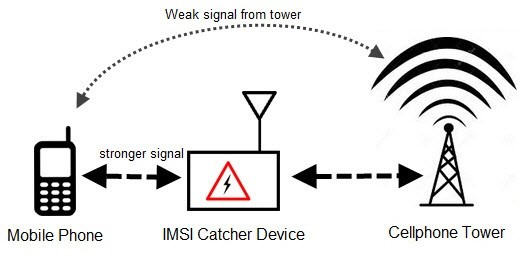
\includegraphics[width=0.5\textwidth]{images/imsi-catcher.jpg}
    \caption{Strumento per rubare IMSI}
\end{figure}\\
Per rubare l'\gls{imsi} si mette in pratica un attacco di tipo \textit{Man In The Middle} (MITM), intromettendosi nella comunicazione fra il \gls{ms} e la \gls{bs}.\\
Nelle reti di seconda generazione questo risulta molto semplice poichè, come spiegato nella sezione 5.1, l'\gls{imsi} viene trasmesso in chiaro se il \gls{ms} è la prima volta che si connette al registro di quella specifica
zona. Inoltre, dato che nel \gls{gsm} l'autenticazione non è mutua è possibile creare una \textit{fake basestation} e collezzionare tutti gli \gls{imsi} dei dispositivi che si connettono.
Sono stati introdotti diversi identificativi temporanei come il \gls{tmsi} per fare in modo che l'\gls{imsi} non debba essere inviato in ogni procedura di autenticazione, ma sono tutti facilmente raggirabili poichè cambiano con una
frequenza troppo bassa.\\
In \cite{dos-imsi} viene illustrato un metodo per ottenere gli \gls{imsi} di qualsiasi dispositivo nello standard UMTS nonostante l'autenticazione mutua. Infatti viene spiegato come basti mandare al \gls{ms} una \textit{user identity request} impersonandosi 
la \gls{vlr} e il \gls{ms} risponderà con il proprio \gls{imsi} in chiaro.
\begin{figure}[h]
    \centering
    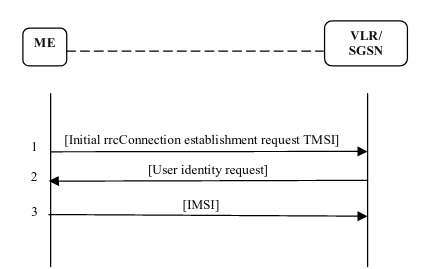
\includegraphics[width=0.5\textwidth]{images/imsi-catch-umts.png}
    \caption{IMSI \textit{catching} nelle reti UMTS\cite{dos-imsi}}
\end{figure}\\

\clearpage

\section{Attacco alle reti con dispositivi SIM-less}
In \cite{umts-dos} e \cite{gsm-dos-simless} sono descritti degli attacchi all'autenticazione degli utenti utilizzando dispositivi senza una \gls{sim} commerciale, ma bensì delle interfacce di comunicazione 
programmabili. Questo è stato fatto perchè utilizzare dei \gls{ms} come dispositivi per effettuare un attacco \gls{dos} rappresenta un fattore limitante in termini di prestazioni. Infatti, 
i sistemi operativi dei \gls{ms} impongono degli intervalli di tempo fra una richiesta e un'altra.\\
Entrambi gli attacchi dimostrano che è possibile causare un \gls{dos} con un numero di dispositivi senza \gls{sim} molto minore rispetto allo stato dell'arte. 
\subsection{GSM}
É stato necessario analizzare la rispettiva \textit{air interface} del \gls{gsm} per valutare quale è il numero massimo di richieste di autenticazione 
che possono essere inviate al secondo a una \textit{base station}. Questa misurazione risulta di fondamentale importanza poichè riesce anche a fornire il numero necessario 
di dispositivi per raggiungere il massimo delle \gls{tps}.
Nell'immagine seguente vengono illustrati i messaggi e i canali in cui viaggiano durante l'autenticazione alla rete \gls{gsm}.
\begin{figure}[h]
    \centering
    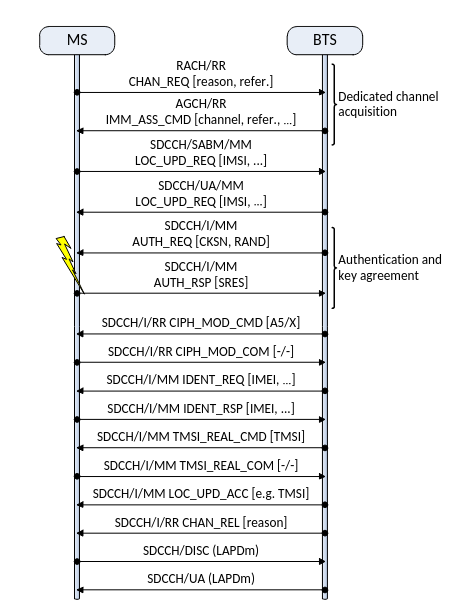
\includegraphics[width=0.5\textwidth]{images/gsm-air-channel.png}
    \caption{Messaggi scambiati durante l'autenticazione in una rete GSM\cite{gsm-dos-simless}}
\end{figure}

\clearpage

\subsection{UMTS}
L'immagine seguente rappresenta un semplice schema del dispositivo con \gls{sim} programmabile per effettuare un \gls{dos} a una rete \gls{umts}\cite{umts-dos}.
\begin{figure}[h]
    \centering
    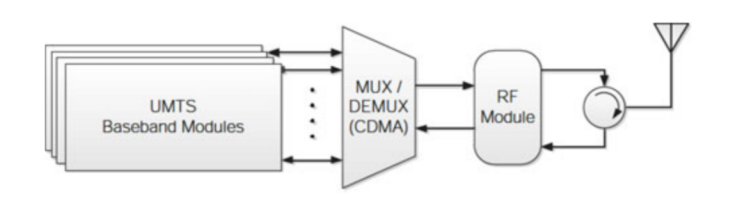
\includegraphics[width=0.5\textwidth]{images/umts-dos-device.png}
    \caption{Dispositivo per l'attacco DOS alle reti UMTS\cite{umts-dos}}
\end{figure}\\
Come è stato fatto per la rete \gls{gsm}, è stato necessario analizzare l'\textit{air interface} dell'\gls{umts} per valutare il numero di \gls{tps}.
Nell'immagine seguente vengono illustrati i messaggi e i canali in cui viaggiano durante l'autenticazione alla rete \gls{umts}.
\begin{figure}[h]
    \centering
    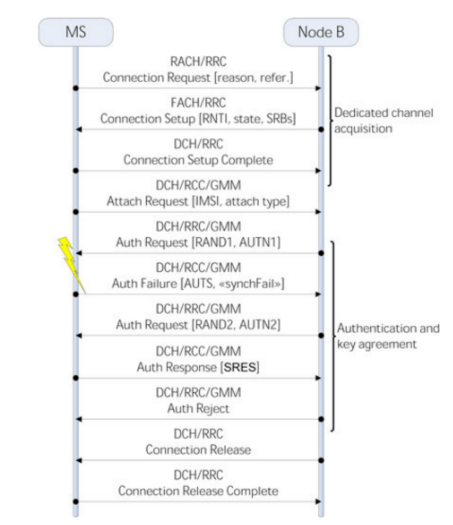
\includegraphics[width=0.5\textwidth]{images/umts-air-channel.png}
    \caption{Messaggi scambiati durante l'autenticazione in una rete UMTS\cite{umts-dos}}
\end{figure}\\
Nelle reti \gls{umts} è stato calcolato che il limite più stringente di TPS durante la comunicazione con la \textit{base station} è dato dal canale \gls{fach} con 28 \gls{tps}.
Questo, ha portato a concludere che bastano 446 dispositivi per effettuare una notevole degradazione del sistema, molti di meno rispetto degli 11K necessari per una \textit{botnet}\cite{dos-imsi}.\\
Nello stesso articolo è spiegato come è possibile duplicare le prestazioni dell'attacco usando delle \gls{sim} valide. In questo modo infatti, i vettori di autenticazione vengono generati una seconda volta se si segnala al
\textit{network} che l'\gls{autn} calcolato non risulta corretto.

    \clearpage
    \chapter{Attacco all'autenticazione delle reti 5G}
In questa sezione verranno trattate le vulnerabilità riguardo un attacco di tipo \gls{dos} all'autenticazione delle reti 5G.
Questa generazione ha risolto alcune delle probematiche legate all'autenticazione, come per esempio a differenza del 4G, l'identificatore 
del \gls{ms} viene criptato con la chiave pubblica prima di essere inviato al \textit{core network}, evitando così di poter essere intercettato e rubato\cite{5g-vs-4g}.
Però, con il grande aumento di dispositivi connessi nel mondo dell' \gls{iot}, gli attacchi \gls{dos} saranno senz'altro più 
semplici da realizzare.\\
I \gls{sdn} e \gls{nfv}, componenti fondamentali per garantire le eccezionali prestazioni del 5G, potrebbero essere un efficace strumento di monitoraggio per identificare possibili 
attacchi come spiegato in \cite{dos-detection-with-sdn}.\\
Allo stesso tempo però, la centralizzazione del controllo del \textit{network} con un \gls{sdn} e \gls{nfv} crea le condizioni ottimali per effettuare un attacco \gls{dos} con successo\cite{5g-dos}.\\
Questa tipologia di attacchi, che ha lo scopo di creare una interruzione del servizio, assume una pericolosià maggiore in questa generazione. Infatti, il mondo dell'\gls{iot} e delle \textit{smart cities} comprendono 
ambiti molto sensibili come per esempio la telemedicina.

\clearpage

\section{IMSI \textit{catching}}
Come anticipato, l'avanzamento più importante in termini di sicurezza che questa nuova generazione ha apportato è sicuramente la trasmissione dell'identificativo del \gls{ms} in forma 
criptata. Questa innovazione ha reso molto più difficile la pratica dell'\gls{imsi} \textit{catching} trattata nella sezione 6.2, fondamentale per effettuare un attacco \gls{dos}.\\
Realisticamente però bisogna sottolineare che questa pratica non risulta completamente debellata. Infatti, tutte le nuove reti 5G, come è stato anche per le generazioni precedenti, devono 
essere retro compatibili, e quindi per un non determinato lasso di tempo devono essere supportate le procedure degli \textit{standard} precedenti che, come spiegato nel capitolo precedente, soffrono 
di questa vulnerabilità.\\
In \cite{suci-catch} viene illustrato un metodo per effettuare un attacco \gls{mitm} nelle reti 5G in modo da ottenere l'\gls{imsi} criptato dell'utente: il \gls{suci}. Questo metodo però non sarebbe applicabile per effettuare 
una raccolta di identificativi per poi effettuare un attacco \gls{dos} poichè il \gls{suci} viene rigenerato dopo ogni utilizzo.
\begin{figure}[ht]
    \centering
    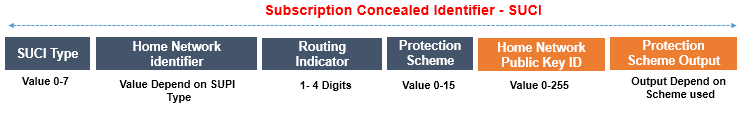
\includegraphics[width=0.8\textwidth]{images/5g-suci.png}
    \caption{Composizione del SUCI nel 5G}
\end{figure}

\section{Replicazione dell'attacco SIM-less}
Alla base degli attacchi trattati nella sezione 6.3 vi è la costruzione di un \textit{database} di \gls{imsi}. Questo \textit{database} può essere agevolmente costruito nelle generazioni precedenti al 5G 
tramite le tecniche di \gls{imsi} \textit{catching} trattate in 6.2. Nel 5G risulta molto più difficile creare un archivio di IMSI poichè questi viaggiano in forma criptata nella rete, ovvero comunicando il \gls{suci}.\\
Tuttavia, se si riuscisse a ottenere comunque un \textit{database} di \gls{imsi} rubati si potrebbe ottenere un attacco dello stesso tipo di \cite{gsm-dos-simless} e \cite{umts-dos} con prestazioni migliori 
perchè il nuovo protocollo 5G NR\cite{5g-nr} per l'\textit{air interface} è stato progettato per supportare il \textit{Massive Machine Type Communications} ovvero l'\gls{iot} massivo che richiede latenze molto basse e capacità molto alte.
Per questo, sicuramente le capacità dei canali di comunicazione durante la procedura di autenticazione avrebbero un valore di TPS molto alto, sufficiente a causare un notevole degradamento delle prestazioni.

\section{Nuove vulnerabilità}
L'implementazione del \gls{suci} e \gls{supi} ha risolto, o quantomeno reso molto più complicata la pratica dell'\gls{imsi} \textit{catching}. Allo stesso tempo però ha incrementato il dispendio di risorse durante l'autenticazione
di un dispositivo. Infatti, prima della generazione dei vettori di autenticazione vengono innestate delle procedure per decriptare il \gls{suci} con un algoritmo detto 
\gls{ecies}. 
Questa procedura aumenta inevitabilmente la creazione di possibili DOS all'autentcazione. 
In \cite{5g-lightweight} è descritto un protocollo che permetterebbe di controllare fin dal primo momento se il \gls{ms} ha un \gls{suci} valido senza incorrere nella decriptazione.
    \clearpage
    \chapter{Conclusioni}
In questo documento sono state analizzate le più comuni vulnerabilità che consentono di effettuare un 
attacco di tipo \textit{denial of service} alle reti cellulari. In particolare, sono state analizzate le vulnerabilità nelle autenticazioni 
di tutte le generazioni.\\
Dopo un'attenta analisi dei meccanismi di autenticazione e delle classiche vulnerabilità che vengono usate nelle generazioni 2G-4G, si può finalmente
fare un confronto fra la sicurezza dell'ultima generazione 5G e quelle precedenti.\\
Il 5G ha sicuramente apportato dei consistenti miglioramenti di sicurezza, come ampiamente trattato riguardo la cifratura dell'\gls{imsi}.\\
Nonostante ciò, è innegabile che in questa ultima generazione gli attacchi \gls{dos} saranno molto più semplici da realizzare, ma sopratutto più pericolosi dati
i compiti sensibili che alcuni dispositivi connessi a questa rete dovranno svolgere.
    \clearpage
    \printbibliography[
        heading=bibintoc,
        title={Bibliografia}
    ]
\end{document}